\tab Cu comanda \textbf{git branch} aratam branch-urile disponibile. Cu comanda \textbf{git checkout "nameOfTheBranch"} am facut switch pe branch-ul repsectiv. In branch-ul curent in care ne aflam am creat un fisier <test> in care am scris <test on branch FirstBranch>. Acesti pasi i-am prezentat in urmatorul screenshoot:
\begin{figure}[h]
\centering
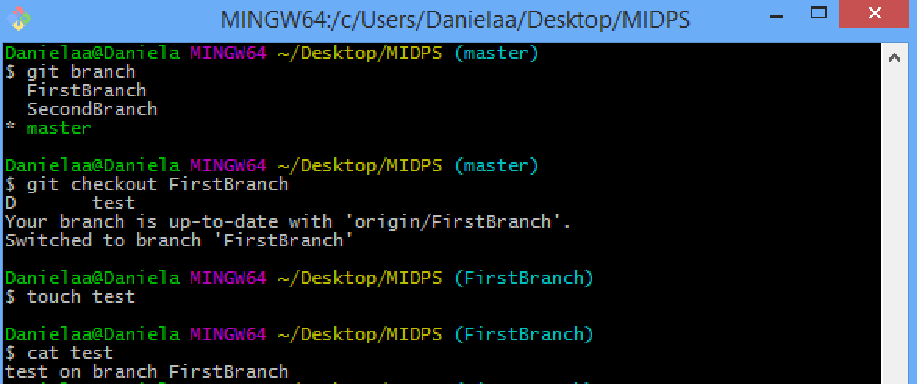
\includegraphics[scale=1]{TestOnFirstBranch}
\end{figure}

\tab Al doilea branch cu vom face conflic este Master , astfel in el am creat la fel un fisier test in care am scris \textbf{test on branch 2}.
In continuare , scriem comanda \textbf{git merge NameOfTheBranch} , si prin urmare obtinem conflict din cazua diferentelor care le-am creat intentionat.
\begin{figure}[h]
\centering
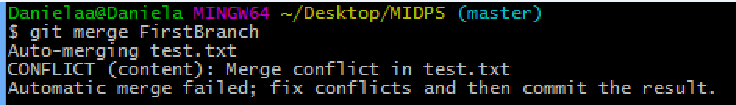
\includegraphics[scale=1]{Conflict.pdf}
\end{figure}

\tab Acum comanda \textbf{git mergetool} ne arata care fisier are conflict si urmeaza a fi merge-uit :D Intradevar fisierul \textbf{test.txt} este cu pricina.
\begin{figure}[h]
\centering
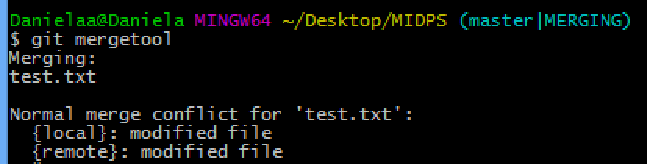
\includegraphics[scale=1]{mergetool.pdf}
\end{figure}
\clearpage